% ----------------------------------------------------------
\chapter{QMDD}
% ----------------------------------------------------------
Quantum Multiple-Valued Decision Diagram é uma estrutura de dados composta de um grafo dirigido acíclico cujos vértices são rotulados para representar um dos qubits do circuito. Por meio dessas informações, é possível percorrer o grafo de forma a reconstruir completamente a matriz que ele representa. Assim, o QMDD se mostra uma forma sem perdas de compactar matrizes. Além disso, é possível manipular QMDDs e realizar operações como adição e multiplicação entre eles sem precisar reconstruir suas matrizes, fazendo com que essas operações também tirem vantagem da capacidade de compressão oferecida pelo QMDD.

Como estabelecido na seção \ref{sec:matrixrep}, para que um circuito quântico possa ser convertido em matrizes para ser simulado, são necessárias 3 operações fundamentais: construção da matriz a partir da porta; multiplicação de matrizes; medição. Nesta seção, serão apresentados os algoritmos necessários para realização dessas operações, em conjunto das subrotinas necessárias para os algoritmos. Por exemplo, a multiplicação de QMDDs faz uso da subrotina de adição de QMDDs.

Além disso, também será feita uma breve introdução ao conceito de grafos, e como eles oferecem formas eficazes de percorrer dados por meio de caminhos, uma funcionalidade essencial para a manipulação e recuperação das informações contidas em QMDDs.

% ----------------------------------------------------------
\section{Grafos}\label{sec:graph}
% ----------------------------------------------------------

QMDDs são grafos dirigidos acíclicos nos quais cada vértice possui um número fixo de arestas, de acordo com as dimensões da matriz que ele representa, e com rótulos para cada vértice. Esta seção busca introduzir conceitos fundamentais para grafos de forma que a definição de um QMDD seja clara. %TODO: rewrite this because I don't know how to say "to make it easier 4 u to understand"

Grafo é o nome dado para estruturas de dados organizadas em elementos e ligações entre esses elementos. Cada elemento do grafo é chamado de vértice e as ligações entre os elementos são chamadas de arestas. Um cenário no qual grafos são úteis, por exemplo, é a representação entre diferentes pontos de ônibus de uma cidade e a existência de uma rota que ligue 2 pontos. Nesse caso, cada ponto de ônibus é um vértice e sempre que exista uma linha de ônibus levando de um ponto A para um ponto B, vai existir uma aresta ligando os vértices A e B. Arestas podem ser representadas como uma tupla com o vértice de saída e o vértice destino da aresta.

O grafo \ref{fig:graph2nodes} é composto do conjunto de vértices \{A, B\} e do conjunto de arestas \{(A, B)\}

\begin{figure}[h]
\centering
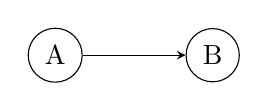
\begin{tikzpicture}[>=stealth, node distance=2cm]

\node (A) [circle, draw] {A};
\node (B) [circle, draw, right of=A] {B};

\draw[->] (A) -- (B);

\end{tikzpicture}
\label{fig:graph2nodes}
\end{figure}


\subsection{Caminhos}
A existência de uma aresta saindo de A e levando a B significa que existe um caminho de A para B. Nem todos os vértices do precisam estar diretamente ligados por uma aresta, é possível que exista um caminho indireto entre dois vértices. Por exemplo, no grafo~\ref{fig:graph3node}, existe um caminho de A para B e um de B para C, isso significa que, indiretamente, também existe um caminho de A para C.

\begin{figure}[h]
\centering
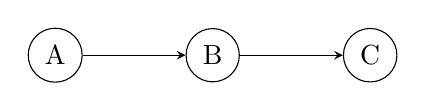
\begin{tikzpicture}[>=stealth, node distance=2cm]

\node (A) [circle, draw] {A};
\node (B) [circle, draw, right of=A] {B};
\node (C) [circle, draw, right of=B] {C};

\draw[->] (A) -- (B);
\draw[->] (B) -- (C);

\end{tikzpicture}
\label{fig:graph3node}
\end{figure}

\subsection{Arestas Ponderadas}
Além de armazenar apenas a informação de que se existe ou não um caminho entre dois vértices, uma aresta também pode armazenar um valor para esse caminho. Normalmente esse valor é entendido como o custo da aresta, porém, nos QMDDs, esse valor é interpretado como um dos valores que compõem a matriz representada.

No exemplo dos pontos de ônibus, o valor de uma aresta poderia representar o tempo que leva para chegar de um lugar a outro. Isso se torna útil em junção com o conceito de caminho indireto: se o caminho de A para C é na verdade o caminho de A para B seguido do caminho de B para C, sabe-se que o custo para chegar em C a partir de A será a soma dos custos para ir de A a B e de B a C. Por exemplo, se a aresta (A, B) tem valor 10 minutos e a aresta (B, C) tem valor 20 minutos, sabe-se que é possível sair de A e chegar em C em 30 minutos.

\begin{figure}[h]
\centering
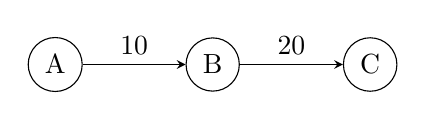
\begin{tikzpicture}[>=stealth, node distance=2cm]

\node (A) [circle, draw] {A};
\node (B) [circle, draw, right of=A] {B};
\node (C) [circle, draw, right of=B] {C};

\draw[->] (A) -- (B) node[midway, above] {10};
\draw[->] (B) -- (C) node[midway, above] {20};

\end{tikzpicture}
\label{fig:graph3nodeweighted}
\end{figure}


\subsection{Grafos Dirigidos e Ciclos}
Note que a possibilidade de ir do ponto A para o ponto B não implica na existência de um caminho de B para A. Por isso a ordem da tupla é importante para as arestas. Dessa forma, grafos podem ou não ser dirigidos, ou seja, é possível impor a restrição de que toda aresta representa a existência de ambos os caminhos, tornando a ordem da tupla irrelevante. Caso o grafo não seja dirigido, toda aresta resulta na existência de um ciclo, ou seja, existe um caminho de um vértice para ele mesmo. No caso da aresta não dirigida (A, B), existe um caminho de A para B e existe um caminho de B para A, logo existe um caminho de A para A.

Por outro lado, no caso de grafos dirigidos, a existência de um ciclo passa a ser apenas uma possibilidade facilmente identificada. No caso dos QMDDs, essa restrição é sempre respeitada pela forma como os algoritmos de construção e manipulação são definidos, porém, dado um grafo arbitrário, é possivel verificar se existe um ciclo por meio de uma busca a partir de cada vértice, verificando se existe um caminho que leve de volta ao mesmo vértice. %TODO: citar busca em profundidade

O grafo \ref{fig:acyclicgraph} é acíclico, visto que não existe caminho de nenhum vértice para si mesmo, já no grafo \ref{fig:cyclicgraph}, existe um caminho de A para A, passando pelos vértices B e C, logo esse grafo é cíclico.

\begin{figure}[h]
\centering
  \begin{minipage}{0.45\textwidth}
    \centering
    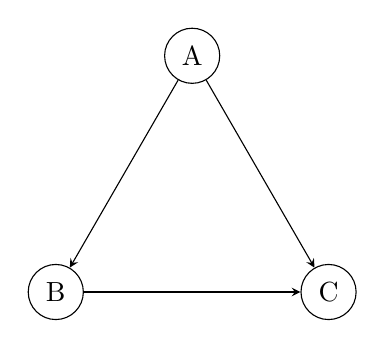
\begin{tikzpicture}[>=stealth, every node/.style={circle,draw,minimum size=7mm}]
      \node (A) at (90:2)  {A};
      \node (B) at (210:2) {B};
      \node (C) at (330:2) {C};
      \draw[->] (A) -- (B);
      \draw[->] (B) -- (C);
      \draw[->] (A) -- (C);
    \end{tikzpicture}
    \label{fig:acyclicgraph}
  \end{minipage}
  \qquad
  \begin{minipage}{0.45\textwidth}
    \centering
    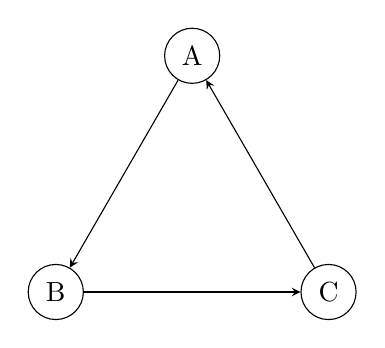
\begin{tikzpicture}[>=stealth, every node/.style={circle,draw,minimum size=7mm}]
      \node (A) at (90:2)  {A};
      \node (B) at (210:2) {B};
      \node (C) at (330:2) {C};
      \draw[->] (A) -- (B);
      \draw[->] (B) -- (C);
      \draw[->] (C) -- (A);
    \end{tikzpicture}
    \label{fig:cyclicgraph}
  \end{minipage}
\end{figure}



% ----------------------------------------------------------
\section{Algoritmos}
% ----------------------------------------------------------

% ----------------------------------------------------------
\subsection{Multiplicação}
% ----------------------------------------------------------

% ----------------------------------------------------------
\subsubsection{Adição}
% ----------------------------------------------------------


% ----------------------------------------------------------
\subsection{Construção a Partir de Portas}
% ----------------------------------------------------------
A construção de um QMDD a partir de uma porta quântica pode ser feita de duas formas possíveis: uma porta arbitrária para um único qubit ou uma porta arbitrária controlada, com um qubit alvo e múltiplos qubits de controle.

A construção de uma porta arbitrária se dá pelo produto tensorial entre matrizes identidade e a matriz que representa a porta arbitrária, de forma a produzir uma única matriz que opere sobre todos os qubits, mantendo todos exceto o qubit alvo da porta inalterados e aplicando o efeito da porta sobre o qubit desejado. Para isso, basta utilizar o algoritmo de produto tensorial definido em \ref{subsub:algkronecker}.
% ----------------------------------------------------------
\subsubsection{Produto Tensorial}
% ----------------------------------------------------------

% ----------------------------------------------------------
\subsubsection{Construção de Portas Controladas}
% ----------------------------------------------------------

% ----------------------------------------------------------
\subsection{Medição}
% ----------------------------------------------------------

% ----------------------------------------------------------
\section{Simulação de Circuitos}
% ----------------------------------------------------------

